\documentclass{article}
\usepackage{graphicx}
\usepackage{hyperref}
\usepackage{enumitem}
\usepackage{datetime}
\usepackage{textcomp}

\usepackage{xcolor}


\begin{document}

\begin{tabular}{@{}ll}
    \textbf{\LARGE Hanxiao Liu} \newline
    \includegraphics*[draft,natwidth=90, natheight=36]{img/name-cn.png}
    &
    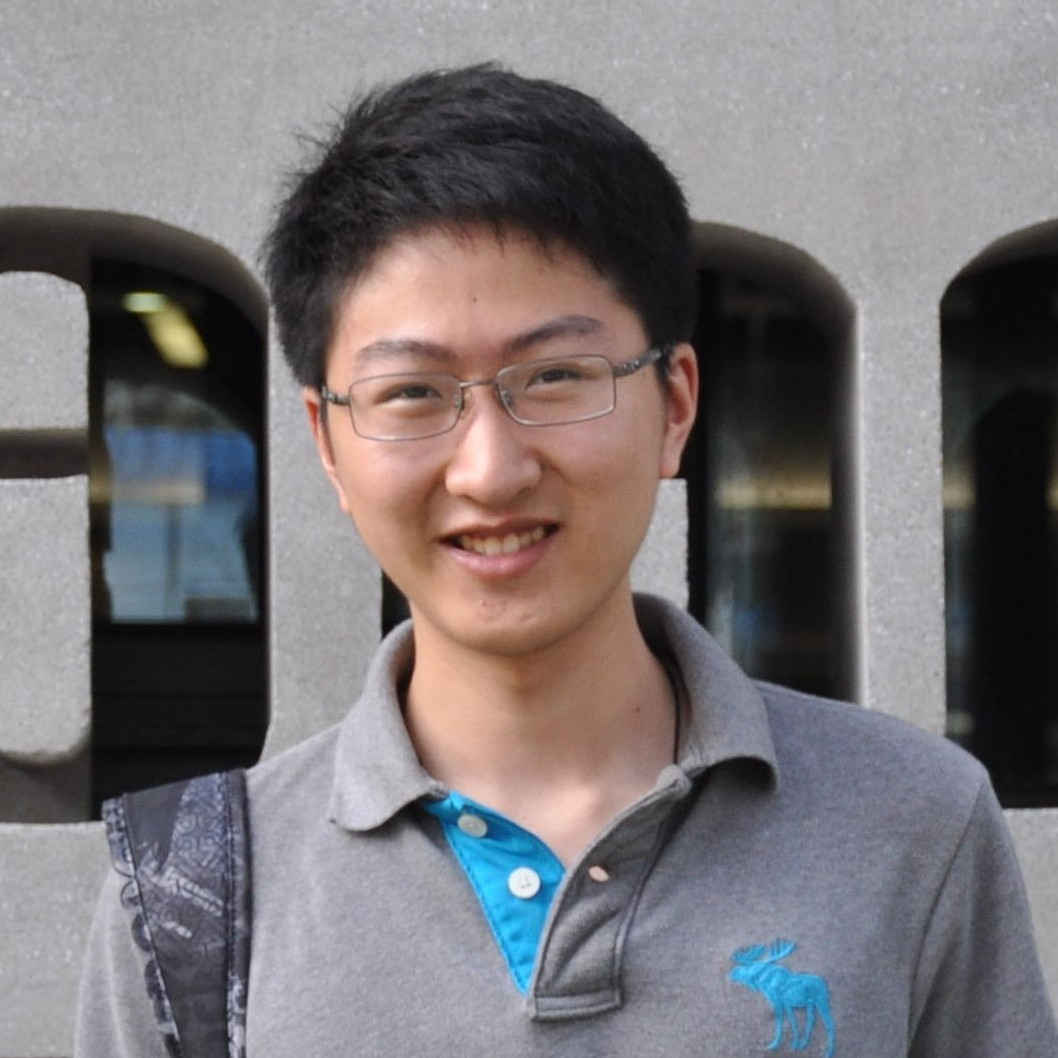
\includegraphics[natwidth=116, natheight=116]{img/profile.jpg} \\
\end{tabular}

\subsection*{--- \protect
\href{https://github.com/quark0}{
\includegraphics[natwidth=24, natheight=24]{img/GitHub-Mark-64px.png}} \
\href{https://scholar.google.com/citations?user=IMkVH_8AAAAJ&hl=en}{
\includegraphics[natwidth=24, natheight=24]{img/google-scholar.png}}
---
}
I am a research scientist at \href{https://ai.google/research/teams/brain}{Google Brain}.

\noindent I received my Ph.D. from
\href{http://www.cmu.edu/index.shtml}{Carnegie Mellon University},
working with Professor \href{http://www.cs.cmu.edu/~./yiming/}{Yiming Yang}.
During my graduate study,
I worked at \href{https://deepmind.com/}{DeepMind} on neural architecture search
and \href{https://www.citadel.com/}{Citadel} on statistical arbitrage.
Prior to that,
I received my B.E.\ from
\href{http://www.tsinghua.edu.cn/publish/newthuen/index.html}{Tsinghua University}.

\noindent My research interest is to build algorithms that learn to learn.

\subsection*{}
\footnotesize{
    \textit{
        Last compiled on \today\ by \href{http://www.tug.org/tex4ht/}{\TeX4ht}. \newline
        Copyright \textcopyright\ \the\year\ Hanxiao Liu. All Rights Reserved.
    }
}

\end{document}
